\documentclass[a4paper, 11pt]{report}
\usepackage{graphicx}
\usepackage{listings}
\usepackage[left=1cm,right=1cm,bottom=2cm,top=2cm]{geometry}
\usepackage{hyperref}

\usepackage{xcolor}
\usepackage{colortbl}
\definecolor{mygreen}{rgb}{0,0.6,0}
\definecolor{mygreen2}{rgb}{0,0.56,0.16}
\definecolor{myred}{rgb}{0.6,0.066,0.066}
\definecolor{mygray}{rgb}{0.5,0.5,0.5}
\definecolor{mymauve}{rgb}{0.58,0,0.82}
\definecolor{mygray}{gray}{0.9}
\definecolor{mywhite}{rgb}{1,1,1}
\definecolor{myblack}{rgb}{0,0,0}
\definecolor{mybeige}{HTML}{eeeeee}

\newcommand{\inlinecode}[1]{\colorbox{mybeige}{\ttfamily\texttt{#1}}}


\lstdefinestyle{code}{ %
  backgroundcolor=\color{mybeige},   % choose the background color; you must add \usepackage{color} or \usepackage{xcolor}; should come as last argument
  basicstyle=\footnotesize\ttfamily,        % the size of the fonts that are used for the code
  breakatwhitespace=false,         % sets if automatic breaks should only happen at whitespace
  breaklines=true,                 % sets automatic line breaking
  captionpos=b,                    % sets the caption-position to bottom
  commentstyle=\color{mygreen},    % comment style
  deletekeywords={...},            % if you want to delete keywords from the given language
  escapeinside={\%*}{*)},          % if you want to add LaTeX within your code
  extendedchars=true,              % lets you use non-ASCII characters; for 8-bits encodings only, does not work with UTF-8
  frame=single,	                   % adds a frame around the code
  keepspaces=true,                 % keeps spaces in text, useful for keeping indentation of code (possibly needs columns=flexible)
  keywordstyle=\color{blue},       % keyword style
  language=Python,                 % the language of the code
  morekeywords={*,...},           % if you want to add more keywords to the set
  numbers=left,                    % where to put the line-numbers; possible values are (none, left, right)
  numbersep=5pt,                   % how far the line-numbers are from the code
  numberstyle=\tiny\color{myblack}, % the style that is used for the line-numbers
  rulecolor=\color{black},         % if not set, the frame-color may be changed on line-breaks within not-black text (e.g. comments (green here))
  showspaces=false,                % show spaces everywhere adding particular underscores; it overrides 'showstringspaces'
  showstringspaces=false,          % underline spaces within strings only
  showtabs=false,                  % show tabs within strings adding particular underscores
  stepnumber=1,                    % the step between two line-numbers. If it's 1, each line will be numbered
  stringstyle=\color{mymauve},     % string literal style
  tabsize=2,	                   % sets default tabsize to 2 spaces
  title=\lstname                   % show the filename of files included with \lstinputlisting; also try caption instead of title
}
\lstset{style=code}

\title{Benchmarks of \texttt{redis-py}, \texttt{hiredis-py} and string creation}
\author{@mokaddem}
\date{\today}

\begin{document}
\maketitle
\tableofcontents
\chapter*{Introduction}
In the course of a software development, I needed a buffering medium which was able to fulfil these requirements:
\begin{itemize}
    \item Capable of handling millions of request per second
    \item Data persistence
    \item Easy to use
\end{itemize}
Where Redis clearly suits them.\\

My software being written in python, I evidently used one of the redis python client available; \texttt{redis-py} is the recommended one.\\

This report focuses only on throughput, so data size was fixed and was fitting my needs.

It contains benchmarks of \texttt{redis-py}, where we can see that it is particularly slow compared to the c-written \texttt{hiredis} library or \texttt{redis-benchmark}. It also presents some features and techniques to boost performances, as well as comparing methods to rapidly create strings.

\chapter{Aggregated results}
\section{Summary}
These tables and plots show a summary for each tested different configuration.
\subsection{Pushing - \texttt{LPUSH}}

\makebox[\textwidth][c]{
    \begin{tabular}{|l|l|c|lll|rrr|}
    \hline
     & \textbf{Tool/feature}        &  \textbf{Parser}        & \multicolumn{3}{c}{\textbf{Total time taken (s)}}  & \multicolumn{3}{|c|}{\textbf{Operation/sec}}  \\
     &  &                & worst & best & average       & worst & best & average        \\
    \hline
    ~\ref{sec:naive} & \multicolumn{1}{c|}{Naive} &  PythonParser  &  2.86 & 2.20 & 2.37   & 34,942 & 45,464 & 42,158     \\
     & \multicolumn{1}{c|}{Naive} &  HiredisParser &  2.20 & 2.09 & 2.17   & 45,388 & 47,745 & 46,150   \\
     & \multicolumn{1}{c|}{Naive} &  hiredis (C)\footnotemark &  1.33 & 1.23 & 1.25   & 75,363 & 81,365 & 79,977   \\
    \hline
    ~\ref{sec:pipeline} & Pipelining \texttt{{\scriptsize -P 1000}}  &  PythonParser  &  1.18 & 1.16 & 1.17   & 85,078 & 85,979 & 85,642    \\
     & Pipelining \texttt{{\scriptsize -P 1000}}  &  HiredisParser &  1.01 & 0.96 & 0.98   & 98,863 & 104,368 & 101,535  \\
     & Pipelining \texttt{{\scriptsize -P 1000}}  &  hiredis (C) &  0.35 & 0.31 & 0.32 & 281,466 & 320,858 & 308,386  \\
    \hline
    ~\ref{sec:cli},~\ref{sec:proto1} & \texttt{redis-cli}, \texttt{format}  &  HiredisParser  &  0.28 & 0.23 & 0.25   & 358,529 & 437,094 & 394,046    \\
    ~\ref{sec:proto2} & \texttt{redis-cli}, \texttt{concatenation +}  &  HiredisParser  &  0.25 & 0.21 & 0.22   & 400,002 & 487,566 & 454,178    \\
    ~\ref{sec:proto3} & \texttt{redis-cli}, \texttt{substitution \%}  &  HiredisParser  &  0.16 & 0.15 & 0.16   & 610,237 & 687,978 & 638,709    \\
    - & \texttt{redis-cli}, (no generation)  &  HiredisParser  &  0.08 & 0.07 & 0.07   & 1,287,382 & 1,523,811 & 1,400,926    \\
    \hline
     & \multicolumn{2}{l|}{\texttt{redis-benchmark {\scriptsize -c 1 -d 129}}} & \multicolumn{3}{c|}{-} & \multicolumn{2}{c}{-} & 117,508 \\
     & \multicolumn{2}{l|}{\texttt{redis-benchmark {\scriptsize -c 1 -d 129 -P 1000 }}} & \multicolumn{3}{c|}{-} & \multicolumn{2}{c}{-} & 1,204,819 \\

    \hline
    \end{tabular}
}
\footnotetext{Official C client}

\subsection{Popping - \texttt{RPOP} or \texttt{LRANGE/LTRIM}}

\makebox[\textwidth][c]{
    \begin{tabular}{|l|l|c|lll|rrr|}
    \hline
     & \textbf{Tool/feature}            & \textbf{parser}        & \multicolumn{3}{c}{\textbf{Total time taken (s)}}  & \multicolumn{3}{|c|}{\textbf{Operation/sec}}  \\
     &                        &               & worst & best & average                & worst & best & average             \\
    \hline
    ~\ref{sec:naive} & \multicolumn{1}{c|}{Naive} &  PythonParser  &  2.68 & 2.11 & 2.27   & 37,301 & 47,323 & 44,021                \\
     & \multicolumn{1}{c|}{Naive} &  HiredisParser &  1.96 & 1.85 & 1.91   & 51,050 & 53,950 & 52,383                  \\
     & \multicolumn{1}{c|}{Naive} &  hiredis (C) &  1.10 & 1.05 & 1.07   & 90,656 & 95,411 & 93,724                  \\
    \hline
    ~\ref{sec:pipeline} & Pipelining              &  PythonParser  &  1.10 & 1.09 & 1.09   & 90,862  & 91,730  & 91,402               \\
     & Pipelining              &  HiredisParser &  0.83 & 0.77 & 0.80   & 121,207  & 129,375  & 124,924                \\
     & Pipelining              &  hiredis (C) &  0.15 & 0.13 & 0.14   & 659,078  & 751,359  & 720,310                \\
    \hline
    ~\ref{sec:lrange} & \texttt{LRANGE} trick   &  PythonParser  &  0.34 & 0.32 & 0.33   & 292,466  & 311,161  & 304,744                \\
     & \texttt{LRANGE} trick   &  HiredisParser &  0.08 & 0.07 & 0.07   & 1,207,644  & 1,511,085  & 1,416,695                \\
     & \texttt{LRANGE} trick   &  hiredis (C) &  0.05 & 0.04 & 0.04   & 2,152,203  & 2,427,007  & 2,318,716                \\
    \hline
     & \multicolumn{2}{l|}{\texttt{redis-benchmark {\scriptsize -c 1 -d 129 (RPOP)}}} & \multicolumn{3}{c|}{-} & \multicolumn{2}{c}{-} & 116,822 \\
     & \multicolumn{2}{l|}{\texttt{redis-benchmark {\scriptsize -c 1 -d 129 -P 1000 (RPOP)}}} & \multicolumn{3}{c|}{-} & \multicolumn{2}{c}{-} & 1,136,363 \\
     & \multicolumn{2}{l|}{\texttt{redis-benchmark {\scriptsize -c 1 -d 129 (LRANGE\_100)}}} & \multicolumn{3}{c|}{-} & \multicolumn{2}{c}{-} & 4,048,000 \\

    \hline
    \end{tabular}
}

\newpage

\begin{minipage}{0.55\linewidth}
    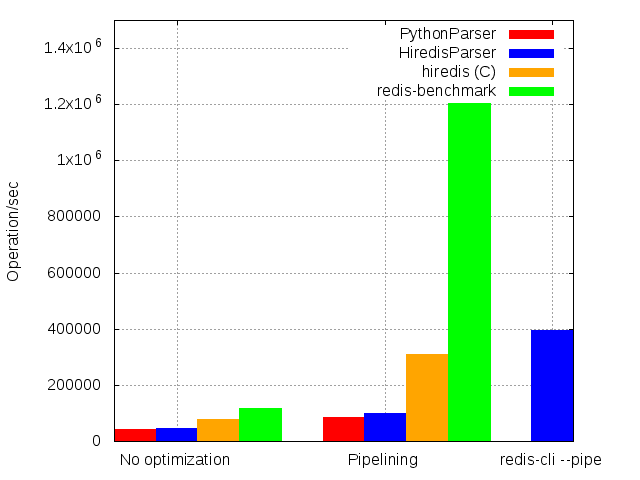
\includegraphics[width=1.07\linewidth]{plots/pushing.png}
\end{minipage}
\begin{minipage}{0.4\linewidth}
    \underline{\texttt{LPUSH:}}\\

    With no optimization, python performs close to 60\% of \texttt{hiredis (C)} performance:
    $$\frac{\texttt{python perf}}{\texttt{hiredis (C) perf}}=\frac{46,150}{79,977}=57.70\%$$
    With pipelining, python performs close to only 30\% of \texttt{hiredis (C)} performance:
    $$\frac{\texttt{python perf}}{\texttt{hiredis (C) perf}}=\frac{101,535}{308,386}=30.91\%$$
\end{minipage}


\begin{minipage}{0.55\linewidth}
    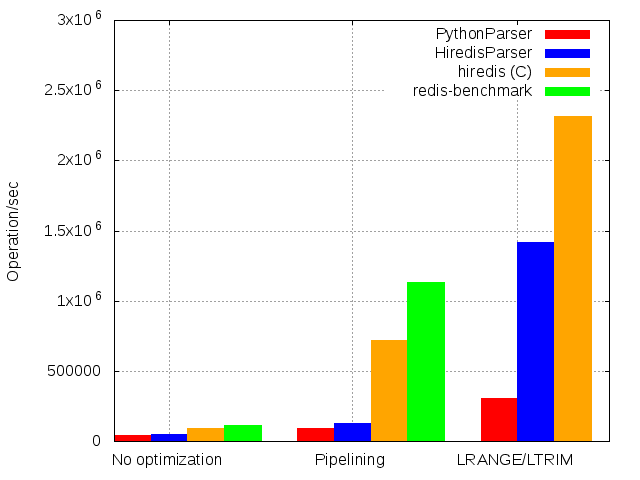
\includegraphics[width=1.0\linewidth]{plots/poping.png}
\end{minipage}
\begin{minipage}{0.4\linewidth}
    \underline{\texttt{POP:}}\\

    With no optimization, python performs close to 60\% of \texttt{hiredis (C)} performance::
    $$\frac{\texttt{python perf}}{\texttt{hiredis (C) perf}}=\frac{52,383}{93,724}=55.89\%$$
    With pipelining, python performs close to only 13\% of \texttt{hiredis (C)} performance:
    $$\frac{\texttt{python perf}}{\texttt{hiredis (C) perf}}=\frac{91,402}{720,310}=12.69\%$$
\end{minipage}


\begin{minipage}{0.55\linewidth}
    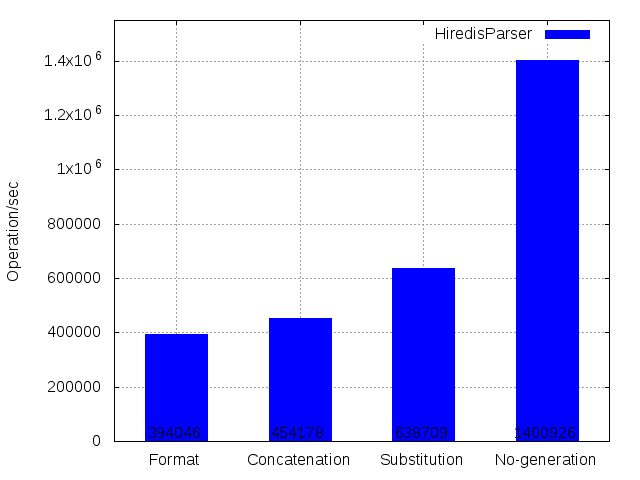
\includegraphics[width=1.0\linewidth]{plots/pushing-proto-algo.png}
\end{minipage}
\begin{minipage}{0.4\linewidth}
    \underline{String Generation:}\\

    \begin{tabular}{|ll|}
        \hline
        Method & Cummulative gain\\
        \hline
        \texttt{format} & 0\%\\
        \texttt{Concatenation} & 15.26\%\\
        \texttt{Substitution} & 40.63\%\\
        \hline
    \end{tabular}
\end{minipage}


\chapter{Detailed implentations and tests}
\section{Benchmark parameters}
All benchmarks have been performed using these parameters
\begin{itemize}
    \item Usage of redis \texttt{unix\_socket\_path}
    \item Payload: size = 129 bytes
        \begin{itemize}
            \item[]
                \begin{lstlisting}
'{"origin": null, "channel": 0, "content": "redis@tshark_save:53619abd-a27c-432c-8f8d-1d059aab5f24", "size": 54, "redirect": true}'
\end{lstlisting}
        \end{itemize}
    \item Operations:
        \begin{itemize}
            \item 100000 \texttt{LPUSH}
            \item Number of \texttt{POP} may differ if we use \texttt{RPOP} or \texttt{LRANGE/LTRIM}
        \end{itemize}
    \item For each tests, we are using two different parsers for responses: PythonParser and HiredisParser\footnote{Hiredis is a C library that is available with Python bindings, \texttt{redis-py} will attempt to use the HiredisParser if you have the hiredis module installed and will fallback to the PythonParser otherwise.}
    \item In order to simulate a working software popping and adding elements to a buffer, the logic of the benchmark is the folloging:
        \begin{itemize}
            \item[] \begin{lstlisting}
# push
# c =   total count     = 100,000
# d =   divisor         = 1,000
# c/d = iteration count = 100
for i in range(int(c/d)):
    for j in range(d):
        # push
    for j in range(d):
        # pop
\end{lstlisting}
        \end{itemize}
        \item For each benchmark, the processing has been done 10 times, then averaged
        \item For each 100 $\left(\frac{100,000}{1,000}\right)$ iterations, we are pushing and popping 1,000 elements
\end{itemize}

%%%
%%% NAIVE
%%%
\newpage
\section{Naive implementation\label{sec:naive}}
For each payload to be buffered, we push them immediatly. Then, we retrieve them one at a time with a simple \texttt{POP} command.\\

\begin{minipage}[t]{0.45\textwidth}
\textbf{Source code}\\
\vspace{-0.5em}
\begin{lstlisting}
# push
t1=time.time()
for j in range(d):
    redis.lpush('k', payload)
    cpush+=1
time_push += time.time()-t1
# pop
t1=time.time()
for j in range(d):
    msg = redis.rpop('k')
    process_message(msg)
    cpop+=1
time_pop += time.time()-t1
\end{lstlisting}
\end{minipage}
\quad
\begin{minipage}[t]{0.5\textwidth}
\textbf{Profiling summary}\\

    \begin{tabular}{|l|l|l|}
        \hline
        Cumulative CPU \% & PythonParser & HiredisParser\\
        \hline
        Processing & 3.95\% & 4.71\%\\
        \hline
        Receiving response & 38.54\% & 28.33\%\\
        \hline
        Sending command & 41.18\% & 48.10\%\\
        \hline
        \multicolumn{3}{|c|}{Parser total gain: \textbf{19.24\%}}\\
        \hline
    \end{tabular}
\end{minipage}

\begin{minipage}[t]{0.5\linewidth}
\textbf{PythonParser}\\

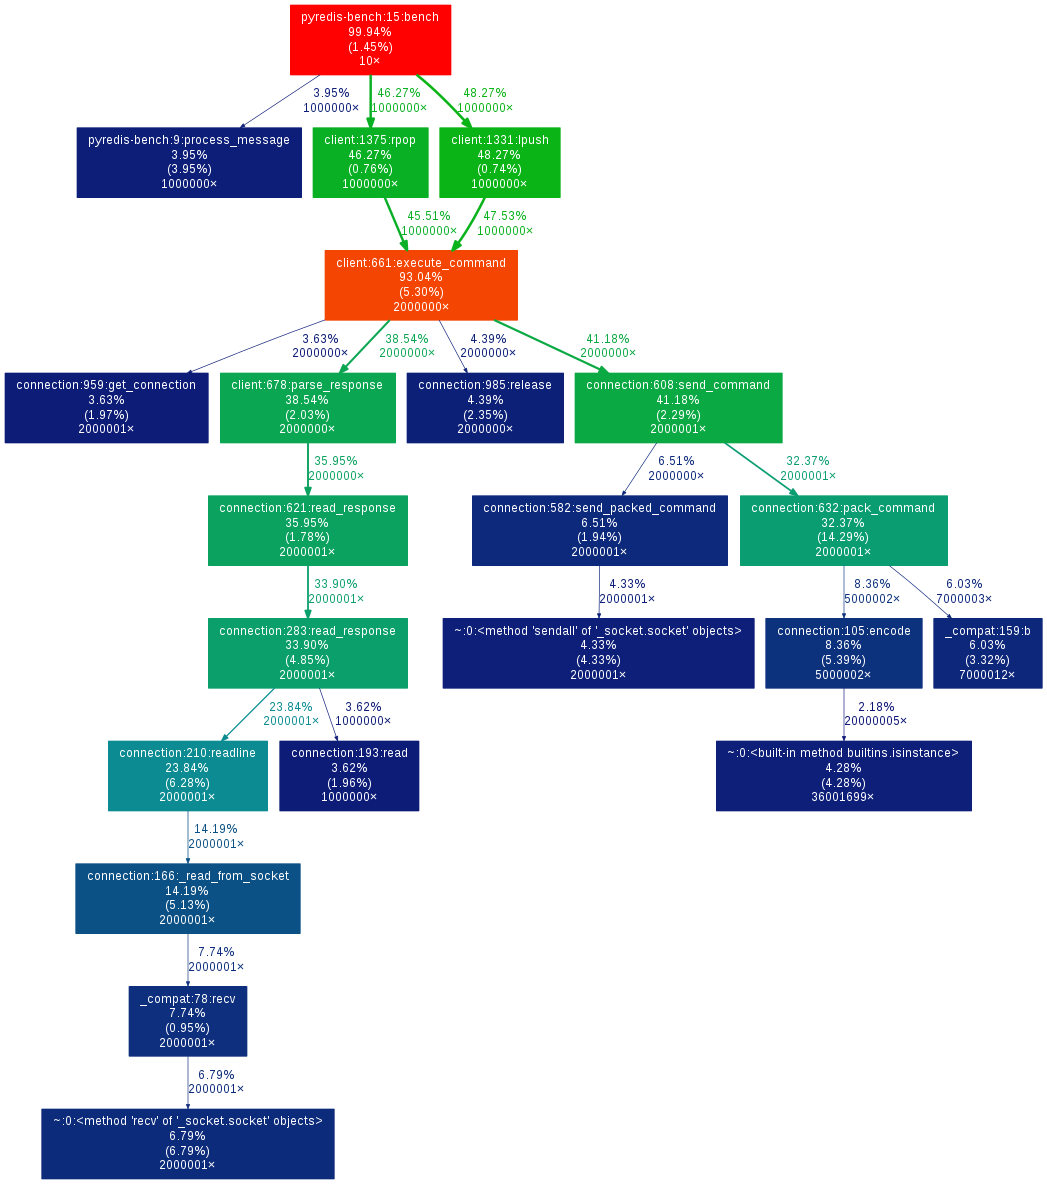
\includegraphics[width=0.9\linewidth]{pics/naive-py.png}
\end{minipage}
\quad
\begin{minipage}[t]{0.5\linewidth}
\textbf{HiredisParser}\\

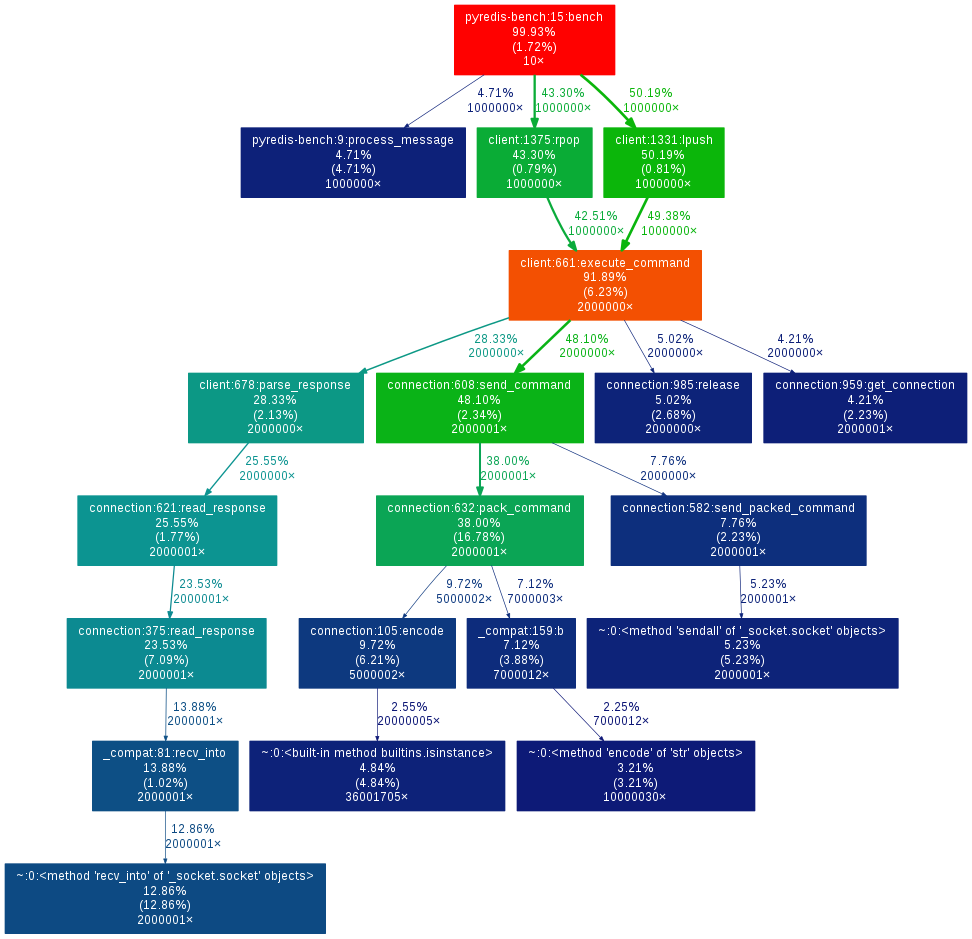
\includegraphics[width=0.9\linewidth]{pics/naive-hi.png}
\end{minipage}

%%%
%%% Pipeline
%%%
\newpage
\section{Pipeline feature\label{sec:pipeline}}
Here, we use the redis pipeline\footnote{Pipelining allows to send multiple commands to the server without waiting for the replies, and finally read the replies in a single step} feature.
For each payload to be buffered, we push them in a pipeline wich will execute pending commands every 1000 pushing operations. Then, we retrieve them by sending the POP command in a pipeline which will also execute pending commands every 1000 popping operations.\\

\begin{minipage}[t]{0.45\textwidth}
\textbf{Source code}\\
\vspace{-0.5em}
\begin{lstlisting}
# push
t1=time.time()
for j in range(d):
    pipeline.lpush('k', payload)
    cpush+=1
pipeline.execute()
tpush += time.time()-t1
# pop
t1=time.time()
for j in range(d):
    pipeline.rpop('k')
resp = pipeline.execute()
for msg in resp:
    process_message(msg)
    cpop+=1
tpop += time.time()-t1
\end{lstlisting}
\end{minipage}
\quad
\begin{minipage}[t]{0.5\textwidth}
\textbf{Profiling summary}\\

    \begin{tabular}{|l|l|l|}
        \hline
        Cumulative CPU \% & PythonParser & HiredisParser\\
        \hline
        Processing & 5.88\% & 7.83\%\\
        \hline
        Receiving response & 35.09\% & 13.90\%\\
        \hline
        Sending command & 47.10\% & 62.91\%\\
        \hline
        Parser total gain: & \multicolumn{2}{c|}{\textbf{33.16\%}}\\
        \hline
        Gain compare to ~\ref{sec:naive}: & \textbf{48.86\%} & \textbf{66.24\%}\\
        \hline
    \end{tabular}
\end{minipage}

\begin{minipage}[t]{0.5\linewidth}
\textbf{PythonParser}\\

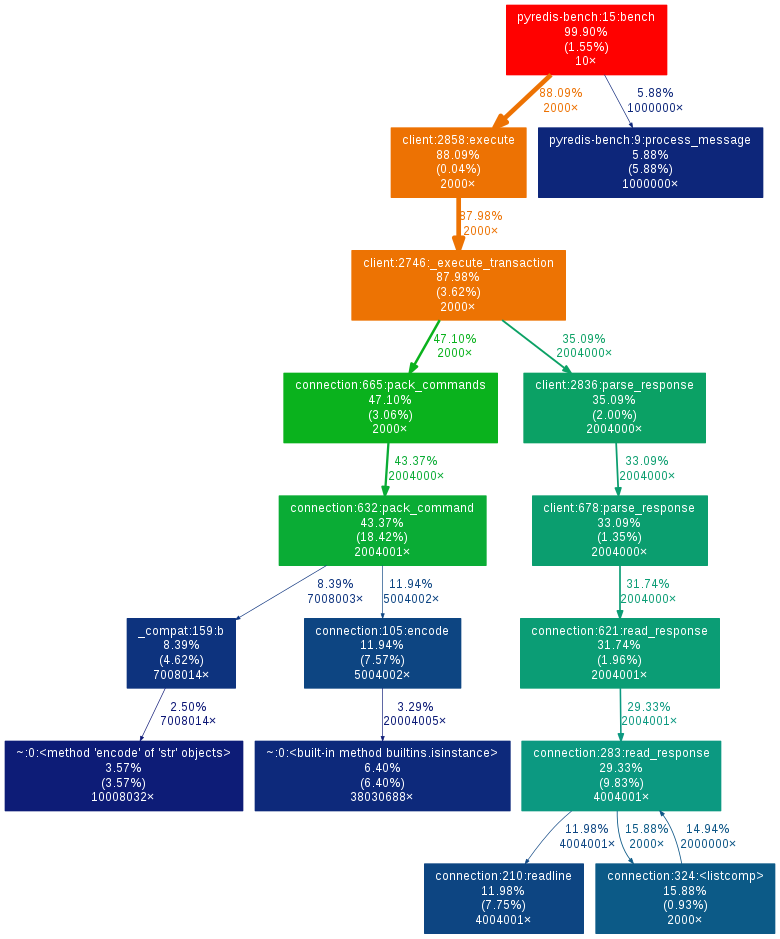
\includegraphics[width=0.9\linewidth]{pics/pipe-py.png}
\end{minipage}
\quad
\begin{minipage}[t]{0.5\linewidth}
\textbf{HiredisParser}\\

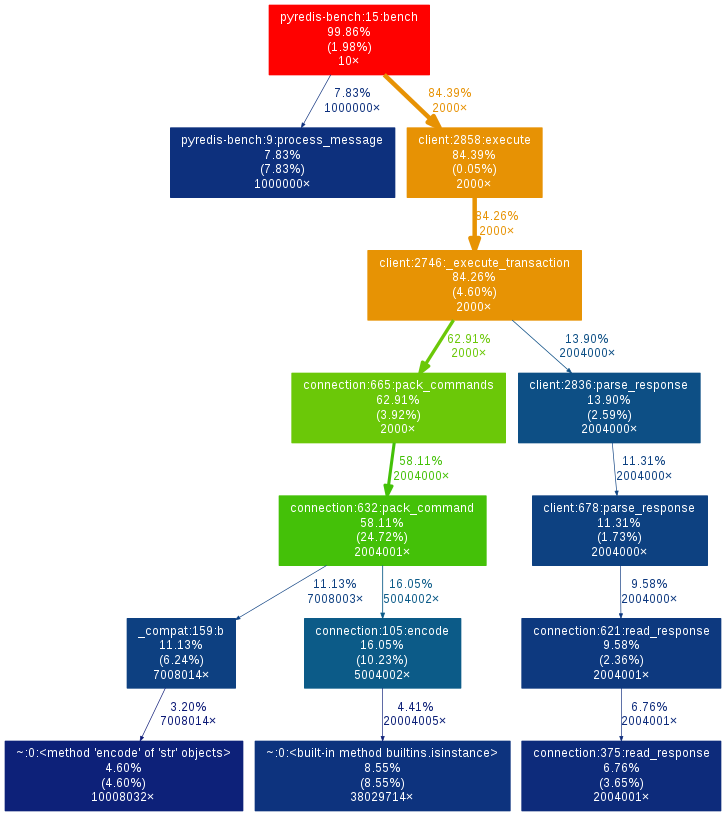
\includegraphics[width=0.9\linewidth]{pics/pipe-hi.png}
\end{minipage}

%%%
%%% LRANGE
%%%
\newpage
\section{Replacing \texttt{RPOP} by \texttt{LRANGE/LTRIM}\label{sec:lrange}}
In this implementation, we are still using the redis pipeline feature for pushing data into the buffer, but we modify the popping behavior.
Instead of sending one POP command at a time to the pipeline, we fetch a range (100 items) of buffered data with \texttt{LRANGE}, then we trim the buffer so that it mirror the effect of a \texttt{POP} command.\\

\begin{minipage}[t]{0.45\textwidth}
\textbf{Source code}\\
\vspace{-0.5em}
\begin{lstlisting}
# lrange_count = 100
# push
t1=time.time()
for j in range(d):
    pipeline.lpush('k', payload)
    cpush+=1
pipeline.execute()
tpush += time.time()-t1
# pop
t1=time.time()
for j in range(int(d/lrange_count)+1):
    msg_list = redis.lrange('k', -lrange_count, -1)
    redis.ltrim('k', 0, -len(msg_list)-1)
    for msg in msg_list:
        process_message(msg)
        cpop+=1
tpop += time.time()-t1
\end{lstlisting}
\end{minipage}
\quad
\begin{minipage}[t]{0.5\textwidth}
\textbf{Profiling summary}\\

    \begin{tabular}{|l|l|l|}
        \hline
        Cumulative CPU \% & PythonParser & HiredisParser\\
        \hline
        Processing & 8.65\% & 12.40\%\\
        \hline
        Receiving response & 37.87\% & 11.67\%\\
        \hline
        Sending command & 40.29\% & 57.52\%\\
        \hline
        Parser total gain: & \multicolumn{2}{c|}{\textbf{43.35\%}}\\
        \hline
        Gain compare to ~\ref{sec:pipeline}: & \textbf{47.11\%} & \textbf{58.37\%}\\
        \hline
    \end{tabular}
\end{minipage}

\begin{minipage}[t]{0.5\linewidth}
\textbf{PythonParser}\\

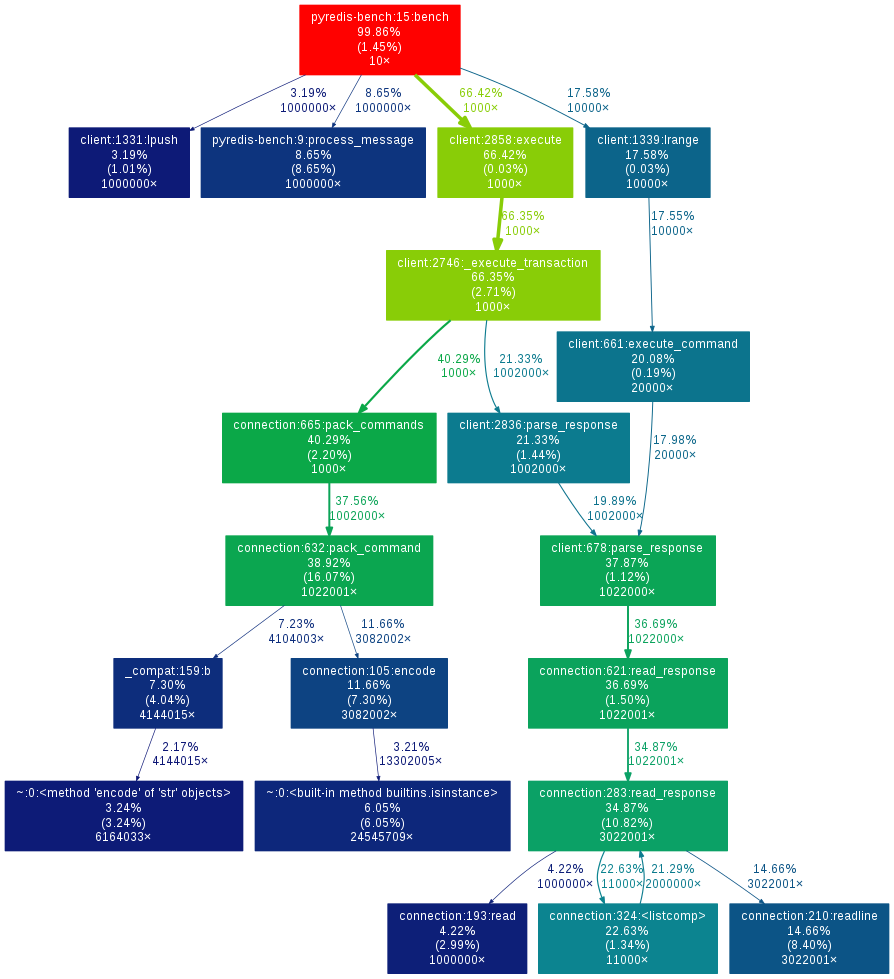
\includegraphics[width=0.9\linewidth]{pics/lrange-py.png}
\end{minipage}
\quad
\begin{minipage}[t]{0.5\linewidth}
\textbf{HiredisParser}\\

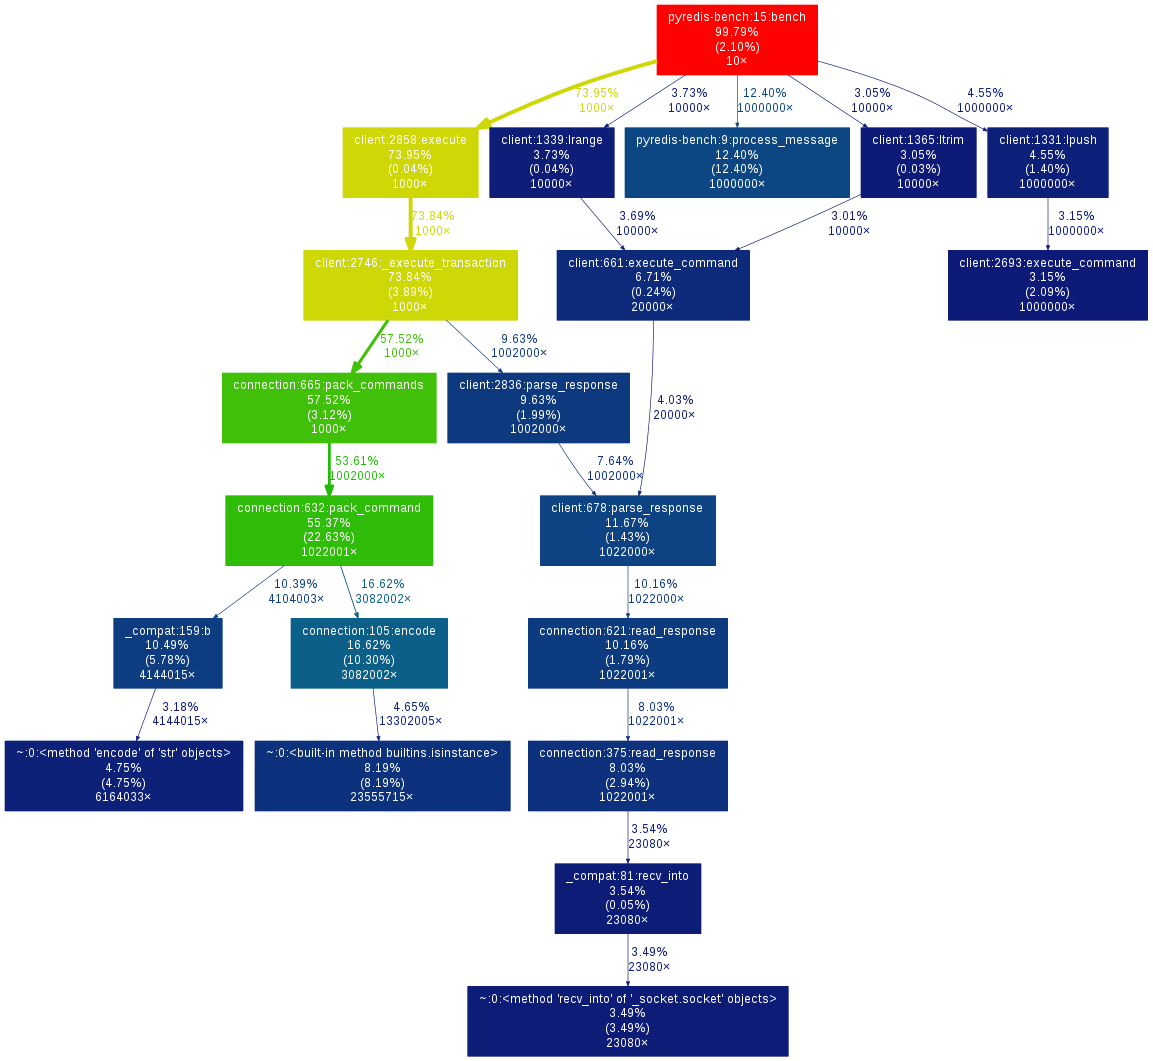
\includegraphics[width=0.9\linewidth]{pics/lrange-hi.png}
\end{minipage}

%%%
%%% REDIS-CLI
%%%
\newpage
\section{Using \texttt{redis-cli --pipe}\label{sec:cli}}
In this implementation, we are still using the redis pipeline feature and the \texttt{LRANGE/LTRIM} replacement of \texttt{POP}. However, we will use the \texttt{redis-cli} binary (provided by redis) with the \inlinecode{--pipe} options\footnote{\texttt{redis-cli --pipe} consists in writing new commands while you read replies at the same time, ignoring the round trip time for every command}.

In order to use this binary, we have to generate the valid redis protocol for the wanted command, which will be written to the STDIN of \texttt{redis-cli}.\\

\begin{minipage}[t]{0.45\textwidth}
\textbf{Source code}\\
\vspace{-0.5em}
\begin{lstlisting}
# push with redis-cli
t1=time.time()
for j in range(d):
    write_to_stdin(generate_redis_protocol('lpush', 'k', payload))
    cpush+=1
tpush += time.time()-t1
# pop with pipeline
t1=time.time()
for j in range(int(d/lrange_count)+1):
    msg_list = redis.lrange('k', -lrange_count, -1)
    redis.ltrim('k', 0, -len(msg_list)-1)
    for msg in msg_list:
        process_message(msg)
        cpop+=1
tpop += time.time()-t1
# flush and close stdin
# pop newly flushed items
\end{lstlisting}
\end{minipage}
\quad
\begin{minipage}[t]{0.5\textwidth}
\textbf{Profiling summary}\\

    \begin{tabular}{|l|l|l|}
        \hline
        Cumulative CPU \% & PythonParser & HiredisParser\\
        \hline
        Processing & 20.50\% & 37.08\%\\
        \hline
        Receiving response & 41.51\% & 6.96\%\\
        \hline
        Sending command\footnote{popping + mass insertion with \texttt{redis-cli}} & 8.45\%\footnote{3.85\% + 4.6\%} & 14.79\%\footnote{6.26\% + 8.53\%} \\
        \hline
        Parser total gain: & \multicolumn{2}{c|}{\textbf{80.87\%}}\\
        \hline
        Gain compare to ~\ref{sec:lrange}: & \textbf{136.99\%} & \textbf{199.03\%}\\
        \hline
    \end{tabular}
\end{minipage}

\begin{minipage}[t]{0.5\linewidth}
\textbf{PythonParser}\\

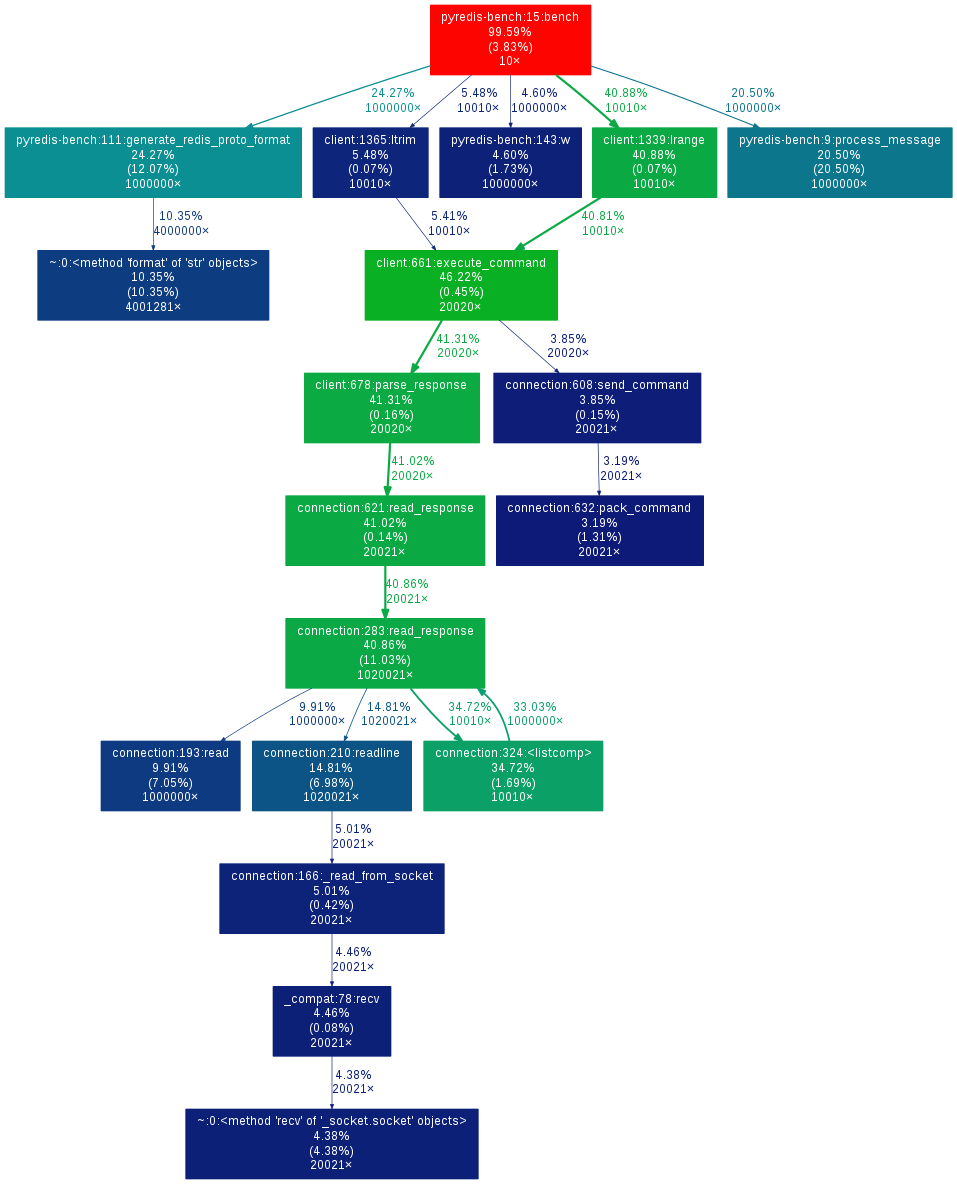
\includegraphics[width=0.9\linewidth]{pics/redis-cli-py.png}
\end{minipage}
\quad
\begin{minipage}[t]{0.5\linewidth}
\textbf{HiredisParser}\\

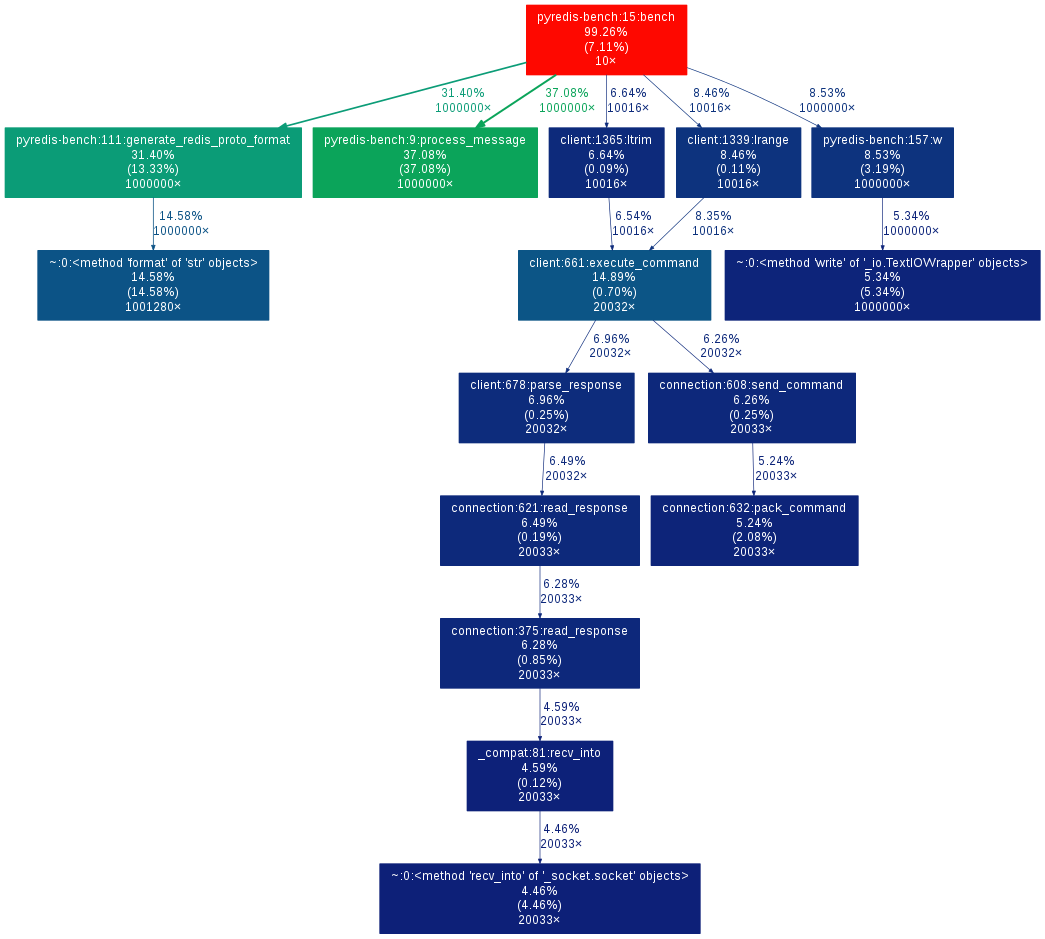
\includegraphics[width=0.9\linewidth]{pics/redis-cli-hi.png}
\end{minipage}


%%%
%%% PROTOCOL
%%%
\newpage
\section{Generating redis protocol\label{sec:proto}}
We saw in section ~\ref{sec:cli} that we need to generate the redis protocol ourself. We will now see differents implentation of doing so, each one with drastically performance improvement.

For each algorythm, we use the same source code as in ~\ref{sec:cli} with the \texttt{HiredisParser}.

\subsection{Generating redis protocol with \texttt{string.Formatter} \label{sec:proto1}}

\begin{lstlisting}
def generate_redis_proto_format(cmd, key, value=''):
    cmd_split = cmd.split()
    if value == '':
        proto = '*{argNum}\r\n${argLen1}\r\n{arg1}\r\n${argLen2}\r\n{arg2}\r\n'.format(
                argNum=3 if value != '' else 2,
                argLen1=len(cmd), arg1=cmd,
                argLen2=len(key), arg2=key
                )
    else:
        proto = '*{argNum}\r\n${argLen1}\r\n{arg1}\r\n${argLen2}\r\n{arg2}\r\n${argLen3}\r\n{arg3}\r\n'.format(
                argNum=3 if value != '' else 2,
                argLen1=len(cmd), arg1=cmd,
                argLen2=len(key), arg2=key,
                argLen3=len(value), arg3=value)
    return proto
\end{lstlisting}

\textbf{Profiling summary}\\
It should be noted that the cumulative CPU time of \texttt{process\_message} entirely depends on the function implentation. Still, it is given as a starting point for comparision.\\

\begin{tabular}{|l|l|}
    \hline
    Cumulative CPU \% & HiredisParser\\
    \hline
    \texttt{process\_message} & 37.08\%\\
    \hline
    \texttt{generate\_redis\_protocol\_format} & 31.40\%\\
    \hline
    Generation \textbf{loss}\footnotemark & \textbf{46.87\%}\\
    \hline
\end{tabular}
\footnotetext{Cost of generating the protocol compated to not generating it a all.}

\subsection{Generating redis protocol with \texttt{String +} concatenation operator\label{sec:proto2}}

\begin{lstlisting}
def generate_redis_proto_concat(cmd, key, value=''):
    cmd_split = cmd.split()
    proto = '*'+(str(3) if value != '' else str(2))+'\r\n'
    proto += '$'+str(len(cmd))+'\r\n'+cmd+'\r\n'
    proto += '$'+str(len(key))+'\r\n'+key+'\r\n'
    if value != '':
        proto += '$'+str(len(value))+'\r\n'+value+'\r\n'
    return proto
\end{lstlisting}

\textbf{Profiling summary}\\

\begin{tabular}{|l|l|}
    \hline
    Cumulative CPU \% & HiredisParser\\
    \hline
    \texttt{processing} & 40.53\%\\
    \hline
    \texttt{generate\_redis\_protocol\_string} & 26.34\%\\
    \hline
    Gain compare to ~\ref{sec:proto1}: & \textbf{9.30\%}\\
    \hline
    Generation \textbf{loss}  & \textbf{34.26\%}\\
    \hline
\end{tabular}


\subsection{Generating redis protocol with \texttt{String \%} substitution operator\label{sec:proto3}}

\begin{lstlisting}
def generate_redis_proto_subst(cmd, key, value=''):
    cmd_split = cmd.split()

    if value != '':
        proto = '*%s\r\n$%s\r\n%s\r\n$%s\r\n%s\r\n$%s\r\n%s\r\n' % ((str(3) if value != '' else str(2)), len(cmd), cmd, len(key), key, len(value), value)
    else:
        proto = '*%s\r\n$%s\r\n%s\r\n$%s\r\n%s\r\n' % ((str(3) if value != '' else str(2)), len(cmd), cmd, len(key), key)
    return proto
\end{lstlisting}

\textbf{Profiling summary}\\

\begin{tabular}{|l|l|}
    \hline
    Cumulative CPU \% & HiredisParser\\
    \hline
    \texttt{processing} & 43.62\%\\
    \hline
    \texttt{generate\_redis\_protocol\_subst} & 19.92\%\\
    \hline
    Gain compare to ~\ref{sec:proto2}: & \textbf{7.62\%} \\
    \hline
    Generation \textbf{loss}  & \textbf{24.85\%}\\
    \hline
\end{tabular}

\chapter*{Conclusion}
We saw that it is not recommended to use \texttt{redis-py} if we need pure throughput. Even so, some features like pipelining or using a different parser increase the performance reasonably, we are still far from those achieved by \texttt{hiredis (C)}.\\

In anycase, using the HiredisParser can increase performances up to 40\% for our case. Don't forget: \texttt{redis-py} uses \texttt{HiredisParser} if it is installed, therefore:\\


\begin{minipage}{0.3\linewidth}
\begin{lstlisting}
pip install redis
pip install hiredis
\end{lstlisting}
\end{minipage}

\end{document}
